\documentclass[11pt]{article}

\usepackage[margin=1in]{geometry}
\usepackage{booktabs}
\usepackage{array}
\usepackage{graphicx}

\title{Summary of Camera-Aware LIBERO Object Experiments}
\author{}
\date{\today}

\begin{document}
\maketitle

\section{Goal}
This note compares an old setting and a new setting for camera-aware LIBERO object experiments, focusing on why the simple variant helps in the old setup but loses to the baseline in the newer \texttt{camtrain60k} setup.

\section{Setup}
Models: \textbf{baseline} = \texttt{pi0\_libero\_pytorch\_full\_finetune}, \textbf{simple} = \texttt{pi0\_libero\_cam\_pytorch\_full\_finetune}, \textbf{standard} = \texttt{pi0\_libero\_cam\_pytorch\_full\_finetune\_standard}.

\begin{table}[h]
\centering
\small
\begin{tabular}{>{\raggedright\arraybackslash}p{3.0cm} >{\raggedright\arraybackslash}p{5.2cm} >{\raggedright\arraybackslash}p{5.2cm}}
\toprule
 & \textbf{Old Setting} & \textbf{New Setting} \\
\midrule
Training dataset & \texttt{glbreeze/libero\_object\_cam} & \texttt{glbreeze/libero\_object\_cam\_train\_o00\_02\_03\_05\_06\_09\_10} \\
Training episodes & 2500 & 4000 \\
Training steps & 30000 & 60000 \\
Models compared & baseline vs. simple & baseline vs. simple vs. standard \\
Evaluation poses & 5 train-distribution poses: \texttt{original}, \texttt{camvar\_00}--\texttt{03}; plus a separate held-out test viewpoint & 12 poses: \texttt{original}, \texttt{camvar\_00}--\texttt{10} \\
Held-out poses in eval & \texttt{camvar\_04}-only, \(\Delta \mathrm{rpy}=(0,6,-60)\) & \texttt{camvar\_01}, \texttt{camvar\_04}, \texttt{camvar\_07}, \texttt{camvar\_08} \\
Trials per task-pose & 50 & 50 \\
Tasks & 10 & 10 \\
Total eval episodes & 2500 + 500 held-out & 6000 \\
\bottomrule
\end{tabular}
\caption{Experiment settings used in this note.}
\label{tab:cam_setup}
\end{table}

For the old setting, we only keep comparisons where baseline and simple are both trained on \texttt{glbreeze/libero\_object\_cam}.

\section{Viewpoints}
Figures~\ref{fig:cam_old_train_views} and~\ref{fig:cam_new_train_views} show the viewpoint coverage of the two settings using real frames.

\begin{figure}[p]
\centering
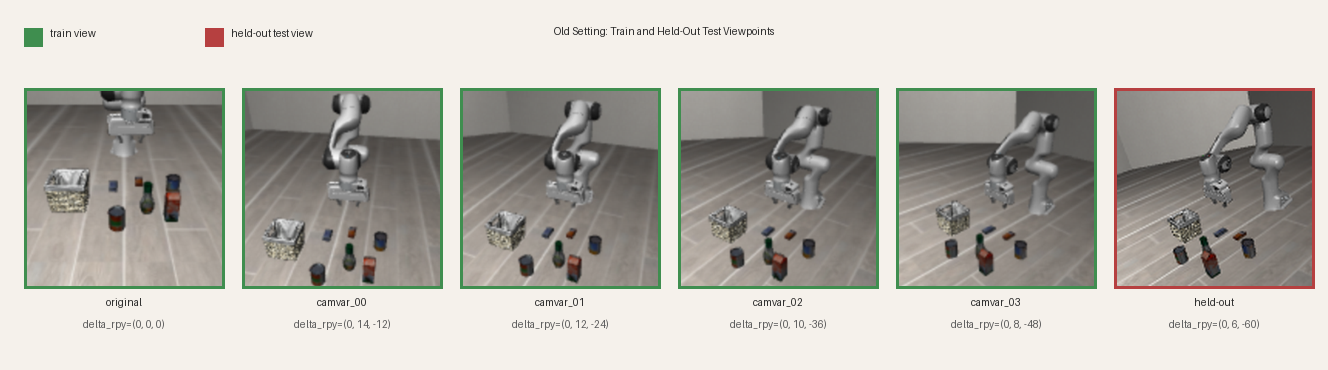
\includegraphics[width=\textwidth]{cam_train_viewpoint_old.png}
\caption{Old setting: five training viewpoints and one held-out test viewpoint (\texttt{camvar\_04}).}
\label{fig:cam_old_train_views}
\end{figure}

\begin{figure}[p]
\centering
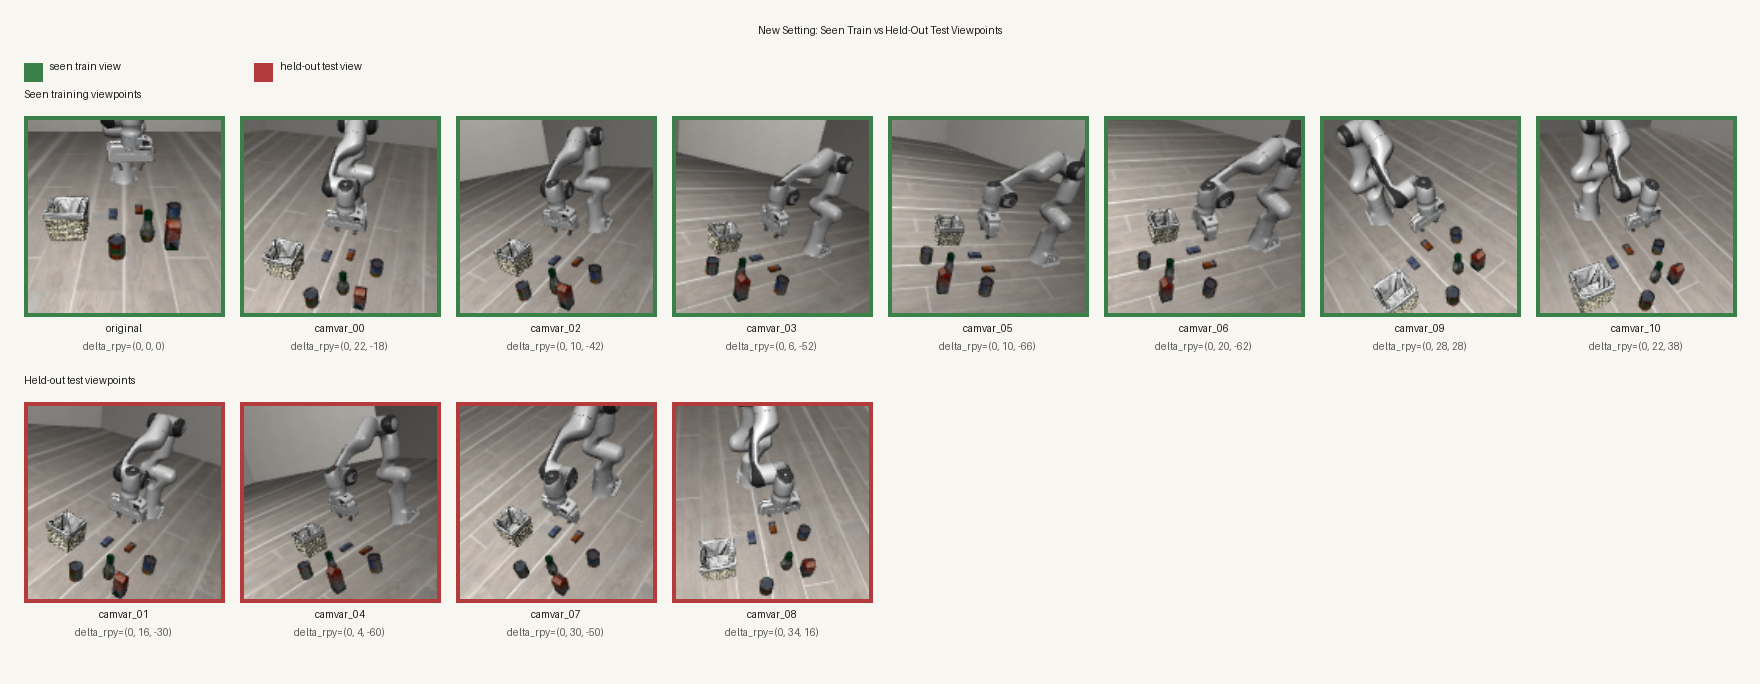
\includegraphics[width=\textwidth]{cam_train_viewpoint_new.png}
\caption{New setting: seen training viewpoints and held-out test viewpoints.}
\label{fig:cam_new_train_views}
\end{figure}

\section{Main Results}
\begin{table}[h]
\centering
\small
\begin{tabular}{lccc}
\toprule
\textbf{Setting} & \textbf{Baseline (\%)} & \textbf{Simple (\%)} & \textbf{Standard (\%)} \\
\midrule
Old: train-distribution poses & 78.8 & \textbf{82.0} & -- \\
Old: held-out test viewpoint & 75.6 & \textbf{79.4} & -- \\
New: overall & \textbf{84.53} & 77.32 & 75.72 \\
\bottomrule
\end{tabular}
\caption{Overall success rates for the old and new settings.}
\label{tab:cam_overall}
\end{table}

The main trend is a sign flip: simple beats baseline in the old setting, but both camera-aware variants trail baseline in the new setting.

\section{Recent Follow-up Experiments}
To isolate which design choice hurts in the new setting, we ran two follow-up experiments after the original \texttt{camtrain60k} comparison:
\begin{itemize}
    \item \textbf{simple\_nocross}: keep the camera pose token, but remove cross-view fusion entirely. This uses the same multi-camera \texttt{camtrain60k} dataset and a two-stage recipe (5k warmup on the new pose module, then joint fine-tuning).
    \item \textbf{relpose\_agentcam\_nocross}: remove fusion as above, switch pose input to relative pose, and rewrite training \texttt{state/actions} into the agent-camera frame before recomputing normalization statistics.
\end{itemize}

\begin{table}[h]
\centering
\small
\begin{tabular}{>{\raggedright\arraybackslash}p{5.1cm}cc>{\raggedright\arraybackslash}p{4.0cm}}
\toprule
\textbf{Experiment} & \textbf{Best ckpt} & \textbf{Success (\%)} & \textbf{Notes} \\
\midrule
Baseline (\texttt{camtrain60k}) & 35000 & \textbf{86.50} & Best result from the original baseline sweep \\
Simple no fusion (\texttt{simple\_nocross}) & 30000 & 85.25 & Same data as \texttt{camtrain60k}; pose token only, no fusion \\
Relative pose + agent-camera action + no fusion & 25000 & 65.50 & Uses rewritten agent-camera-frame actions and new norm stats \\
\bottomrule
\end{tabular}
\caption{Recent follow-up experiments on top of the new setting. Removing cross-view fusion closes most of the gap to baseline, while switching to relative pose plus agent-camera-frame actions performs much worse.}
\label{tab:cam_followup_summary}
\end{table}

These follow-ups suggest that the main regression in the newer camera-aware variants comes from the fusion/action-space design rather than from adding camera conditioning itself. The no-fusion simple variant nearly matches baseline, while the relative-pose camera-frame variant remains far below it.

\section{Checkpoint Sweep Results}
Sweeps are included only to show training dynamics. The old sweep compares \texttt{cam\_pi0\_baseline} and \texttt{posefusion\_multi}, both trained on \texttt{glbreeze/libero\_object\_cam}.

\begin{figure}[p]
\centering
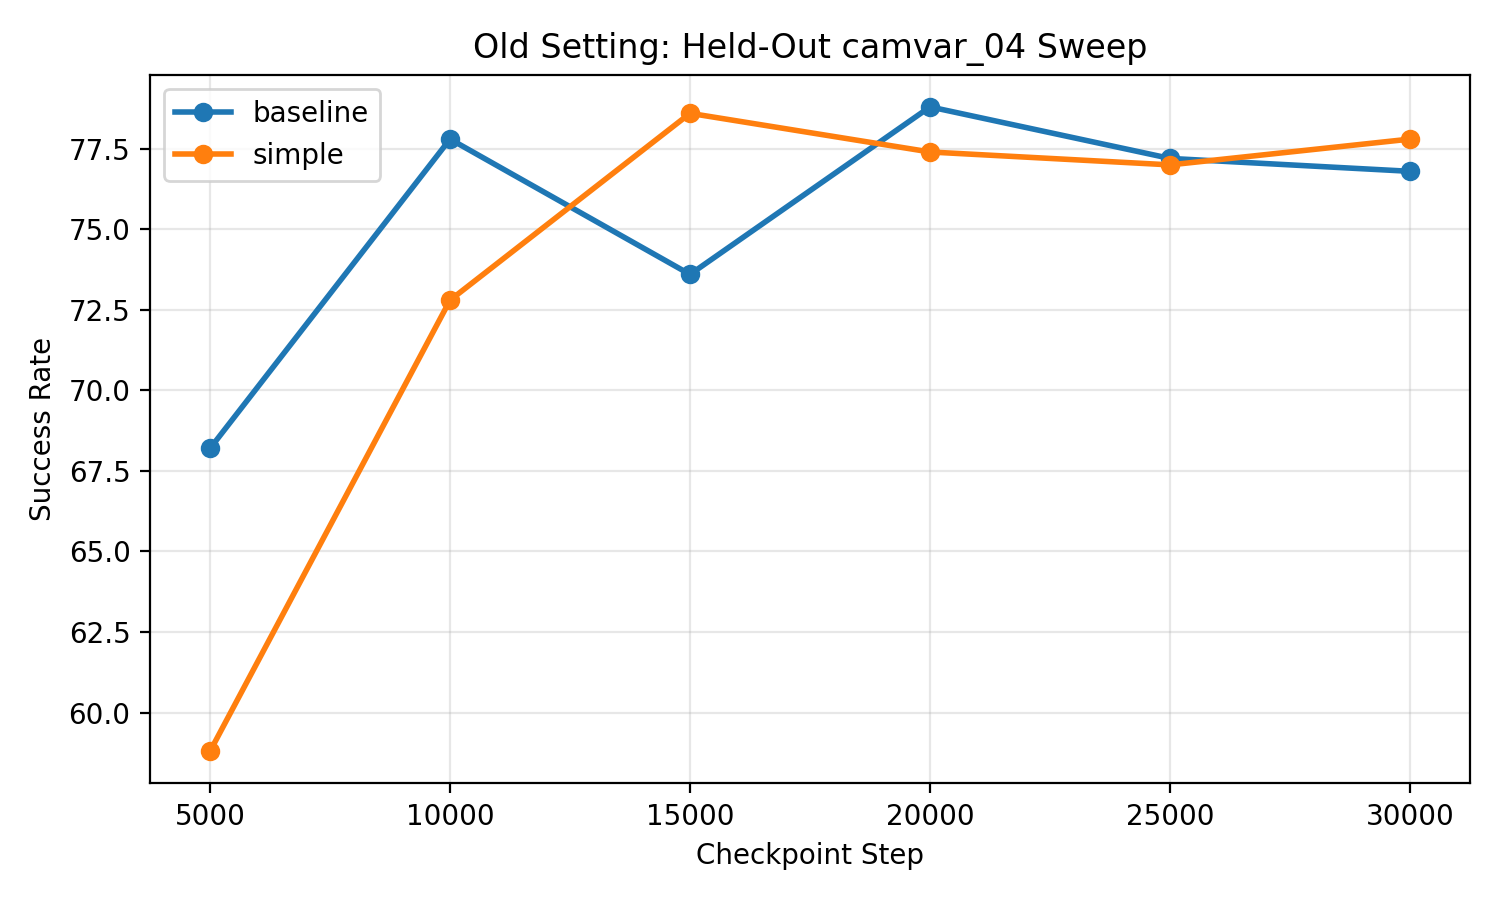
\includegraphics[width=0.82\textwidth]{old_setting_curve.png}
\caption{Old setting held-out \texttt{camvar\_04} checkpoint sweep.}
\label{fig:old_setting_curve}
\end{figure}

\begin{table}[h]
\centering
\small
\begin{tabular}{lcc}
\toprule
\textbf{Step} & \textbf{Baseline (\%)} & \textbf{Simple (\%)} \\
\midrule
5000 & 68.20 & 58.80 \\
10000 & 77.80 & 72.80 \\
15000 & 73.60 & 78.60 \\
20000 & 78.80 & 77.40 \\
25000 & 77.20 & 77.00 \\
30000 & 76.80 & 77.80 \\
\bottomrule
\end{tabular}
\caption{Old setting held-out \texttt{camvar\_04} checkpoint sweep values, using models trained on the original \texttt{glbreeze/libero\_object\_cam} dataset.}
\label{tab:old_setting_curve}
\end{table}

\begin{figure}[p]
\centering
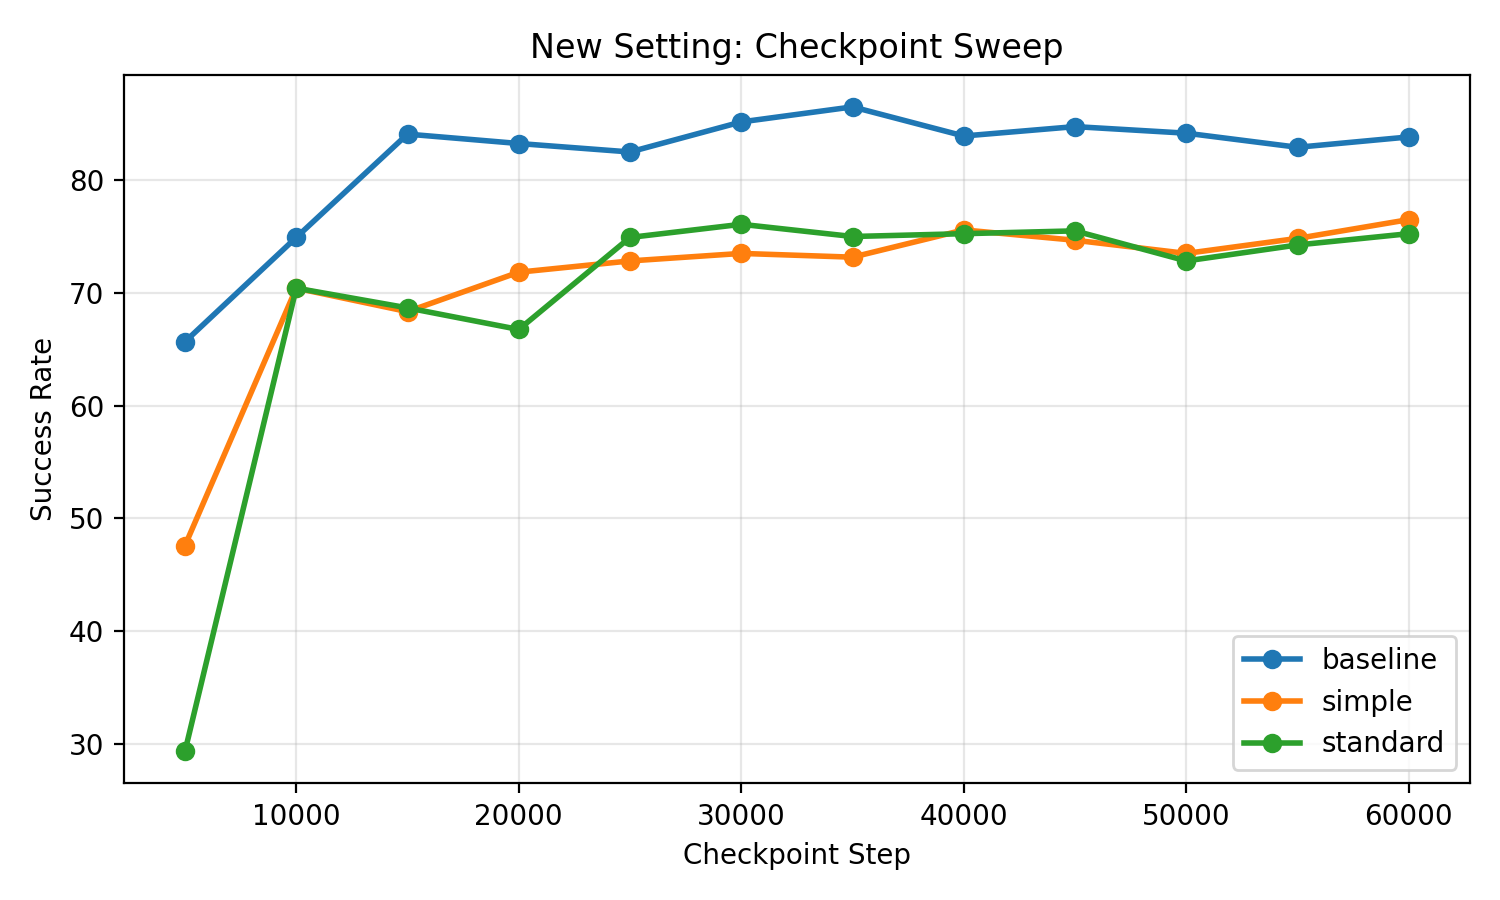
\includegraphics[width=0.9\textwidth]{new_setting_curve.png}
\caption{New setting checkpoint sweep.}
\label{fig:new_setting_curve}
\end{figure}

\begin{table}[p]
\centering
\small
\begin{tabular}{lccc}
\toprule
\textbf{Step} & \textbf{Baseline (\%)} & \textbf{Simple (\%)} & \textbf{Standard (\%)} \\
\midrule
5000 & 65.67 & 47.58 & 29.33 \\
10000 & 74.92 & 70.42 & 70.42 \\
15000 & 84.08 & 68.33 & 68.67 \\
20000 & 83.25 & 71.83 & 66.75 \\
25000 & 82.50 & 72.83 & 74.92 \\
30000 & 85.17 & 73.50 & 76.08 \\
35000 & 86.50 & 73.17 & 75.00 \\
40000 & 83.92 & 75.58 & 75.25 \\
45000 & 84.75 & 74.67 & 75.50 \\
50000 & 84.17 & 73.50 & 72.83 \\
55000 & 82.92 & 74.83 & 74.25 \\
60000 & 83.83 & 76.50 & 75.25 \\
\bottomrule
\end{tabular}
\caption{New setting checkpoint sweep values.}
\label{tab:new_setting_curve}
\end{table}

The sweeps match the full evaluations: the old setting is close and ends slightly in favor of simple, while the new setting is baseline-dominant throughout most of training.

\begin{table}[p]
\centering
\small
\begin{tabular}{lcc}
\toprule
\textbf{Step} & \textbf{Simple no fusion (\%)} & \textbf{RelPose + agent-cam action + no fusion (\%)} \\
\midrule
5000 & 59.00 & 52.75 \\
10000 & 71.25 & 54.33 \\
15000 & 70.42 & 65.00 \\
20000 & 78.08 & 61.58 \\
25000 & 82.25 & \textbf{65.50} \\
30000 & \textbf{85.25} & 62.58 \\
35000 & 81.75 & -- \\
40000 & 82.83 & -- \\
45000 & 80.67 & -- \\
50000 & 82.75 & -- \\
55000 & 83.58 & -- \\
\bottomrule
\end{tabular}
\caption{Checkpoint sweeps for the two recent follow-up experiments. The no-fusion simple variant improves steadily and peaks at 30k, while the relative-pose agent-camera-action variant peaks early at 25k and then degrades.}
\label{tab:cam_followup_curve}
\end{table}

\section{Old Setting Details}
The old setting evaluates five train-distribution poses plus a separate held-out viewpoint, \texttt{camvar\_04}.

\begin{table}[h]
\centering
\small
\begin{tabular}{lcc}
\toprule
\textbf{Pose} & \textbf{Baseline (\%)} & \textbf{Simple (\%)} \\
\midrule
\texttt{original} & 76.00 & 73.40 \\
\texttt{camvar\_00} & 78.20 & 83.40 \\
\texttt{camvar\_01} & 77.00 & 83.80 \\
\texttt{camvar\_02} & 80.20 & 84.60 \\
\texttt{camvar\_03} & 82.60 & 84.80 \\
\bottomrule
\end{tabular}
\caption{Old setting, train-distribution per-pose success rates.}
\label{tab:cam_old_pose}
\end{table}

\begin{table}[h]
\centering
\small
\begin{tabular}{lcc}
\toprule
\textbf{Viewpoint} & \textbf{Baseline (\%)} & \textbf{Simple (\%)} \\
\midrule
\texttt{camvar\_04}-only, \(\Delta \mathrm{rpy}=(0,6,-60)\) & 75.60 & 79.40 \\
\bottomrule
\end{tabular}
\caption{Old setting, held-out test viewpoint results.}
\label{tab:cam_old_heldout}
\end{table}

\section{New Setting Details}
The new \texttt{camtrain60k} setting evaluates 12 poses, with \texttt{camvar\_01}, \texttt{camvar\_04}, \texttt{camvar\_07}, and \texttt{camvar\_08} treated as held-out.

\begin{table}[h]
\centering
\small
\begin{tabular}{lccc}
\toprule
\textbf{Split} & \textbf{Baseline (\%)} & \textbf{Simple (\%)} & \textbf{Standard (\%)} \\
\midrule
Overall & 84.53 & 77.32 & 75.72 \\
Seen poses & 84.53 & 77.60 & 75.62 \\
Held-out poses & 84.55 & 76.75 & 75.90 \\
\bottomrule
\end{tabular}
\caption{New setting, broken down by seen and held-out camera poses.}
\label{tab:cam_current_split}
\end{table}

\begin{table}[p]
\centering
\small
\begin{tabular}{lccc}
\toprule
\textbf{Pose} & \textbf{Baseline (\%)} & \textbf{Simple (\%)} & \textbf{Standard (\%)} \\
\midrule
\texttt{original} & 78.60 & 76.40 & 78.20 \\
\texttt{camvar\_00} & 86.60 & 76.00 & 74.20 \\
\texttt{camvar\_01} & 84.20 & 75.80 & 77.40 \\
\texttt{camvar\_02} & 83.80 & 79.80 & 74.60 \\
\texttt{camvar\_03} & 86.20 & 76.40 & 73.80 \\
\texttt{camvar\_04} & 83.20 & 77.60 & 74.40 \\
\texttt{camvar\_05} & 85.20 & 77.60 & 74.80 \\
\texttt{camvar\_06} & 83.80 & 77.20 & 74.80 \\
\texttt{camvar\_07} & 87.40 & 77.20 & 73.60 \\
\texttt{camvar\_08} & 83.40 & 76.40 & 78.20 \\
\texttt{camvar\_09} & 86.40 & 78.40 & 80.20 \\
\texttt{camvar\_10} & 85.60 & 79.00 & 74.40 \\
\bottomrule
\end{tabular}
\caption{New setting, per-pose success rates.}
\label{tab:cam_current_pose}
\end{table}

\section{Takeaway}
\begin{itemize}
    \item \textbf{Old setting}: simple is slightly better than baseline on both train-distribution poses and the held-out \texttt{camvar\_04} view.
    \item \textbf{New setting}: baseline is clearly better than both camera-aware variants on overall, seen, and held-out poses.
    \item \textbf{Follow-up 1}: removing cross-view fusion nearly recovers baseline performance (85.25\% vs. 86.50\%).
    \item \textbf{Follow-up 2}: moving to relative pose plus agent-camera-frame actions hurts badly; the best checkpoint reaches only 65.50\%.
    \item The main difference is the geometry regime: the old setup is narrow, while the new setup requires broader cross-view generalization.
\end{itemize}

\end{document}
